\section{Auswertung}
\subsection{Die Drillachse}
\subsubsection{Die Winkelrichtgröße}
Um die Winkelrichtgröße $D$ der Drillachse zu bestimmen wird Gleichung
\eqref{eq:D}
verwendet. Die benötigten werte für die Kraft $F$, den Radius $r$ und den Winkel $\phi$ lassen sich der Tabelle \ref{tab:tab1}
entnehmen.
\[D=\SI{2,56(6)e-2}{\joule}\]
\begin{table}
	\centering
	\caption{Messdaten zur Winkelrichtgrößenbestimmung}
	\sisetup{table-format=1.2}
	\begin{tabular}{S[table-format=3.2] S[table-format=3.2]S[table-format=3.2]S[table-format=3.2]}
		\toprule
		{$F/\si[per-mode=reciprocal]{\newton}$}&{$r/\si[per-mode=reciprocal]{\metre}$}&{$\phi/\si[per-mode=reciprocal]{\radian}$} \\
		\midrule
		0,12 & 0,119 & 0,524 \\
		0,19 & 0,119 & 0,873 \\		
		0,38 & 0,059 & 0,873 \\
		0,16 & 0,190 & 1,047 \\
		0,20 & 0,170 & 1,222 \\
		0,30 & 0,110 & 1,396 \\
		0,28 & 0,139 & 1,571 \\	
		0,27 & 0,159 & 1,745 \\
		0,30 & 0,170 & 2,094 \\
		0,22 & 0,239 & 2,269 \\
		\bottomrule
	\end{tabular}
	\label{tab:tab1}
\end{table}
\subsubsection{Eigenträgheitsmoment}
Zur Bestimmung des Eigenträgheitsmoments werden zwei Zylinder mit dem Durchmesser $d = \SI{0,035}{\metre}$, der Höhe $h = \SI{0,03}{\metre}$ und der Masse $m = \SI{0,2218}{\kilogram}$ benutzt.\newline Die Verbindungsstange wird als masselos angenommen und wird daher nicht berücksichtigt.
Die Werte für das Quadrat der Periodendauer $T$ und des Abstands $a$ aus Tabelle \ref{tab:tab2} sind im Graph \ref{fig:abb2} gegeneinander aufgetragen. Mittels linearer Regression ergibt sich hier als Achsenabschnitt \[T_.0^2=\SI{5,0(2)}{\second\squared}\]
Mit Gleichung \eqref{eq:I_D}
ergibt sich für das Trägheitsmoment $I_.D$ der Drillachse:
\[I_.D=\SI{3,2(1)e-3}{\kilogram\metre\squared}\]
\begin{figure}
\centering
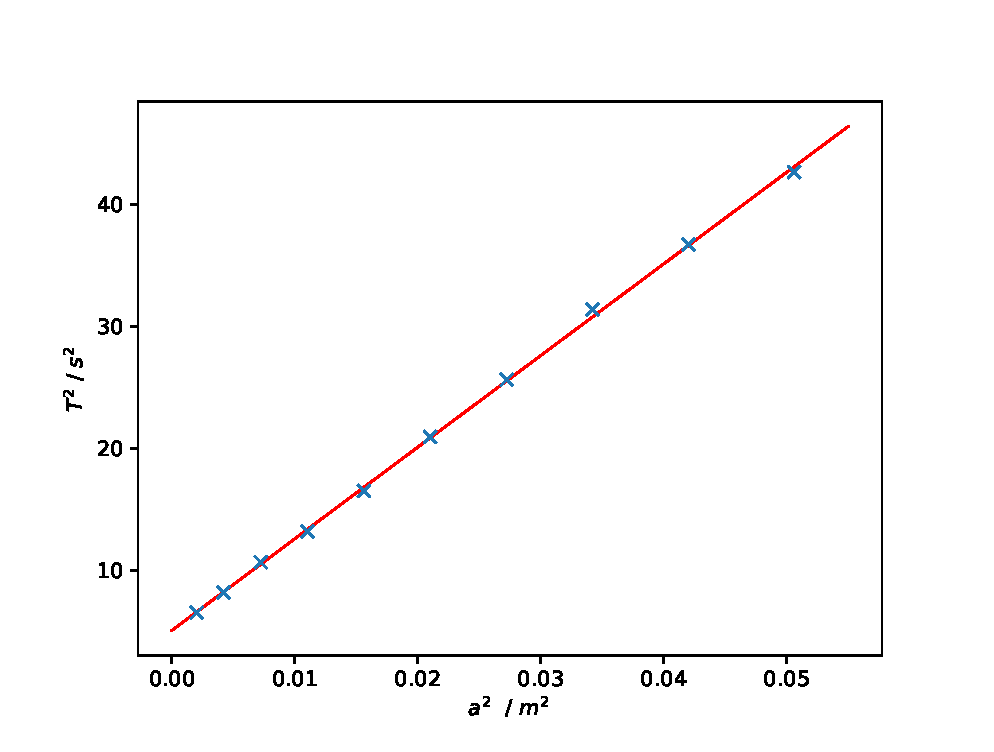
\includegraphics[scale = .75,keepaspectratio]
	{content/images/plot1.eps}
\caption{Graph der Messdaten zur Bestimmung des Eigenträgheitsmoments der Drillachse}\label{fig:abb2}
\end{figure}
\begin{table}
	\centering
	\caption{Messdaten zur Eigenträgheitsmomentbestimmung}
	\sisetup{table-format=1.2}
	\begin{tabular}{S[table-format=3.2] S[table-format=3.2]S[table-format=3.2]S[table-format=3.2]}
		\toprule
		{$r/\si[per-mode=reciprocal]{\metre}$}&{$T/\si[per-mode=reciprocal]{\second}$} \\
		\midrule
		0,045 & 2,5525 \\
		0,065 & 2,86 \\
		0,085 & 3,2675 \\
		0,105 & 3,63 \\
		0,125 & 4,065 \\
		0,145 & 4,575 \\
		0,165 & 5,06 \\
		0,185 & 5,6 \\
		0,205 & 6,06 \\
		0,225 & 6,53 \\
		\bottomrule
	\end{tabular}
	\label{tab:tab2}
\end{table}

\subsection{Das Trägheitsmomentmoment einer Kugel}
\begin{table}
	\centering
	\caption{Messdaten zur Trägheitsmomentbestimmung einer Kugel}
	\sisetup{table-format=1.2}
	\begin{tabular}{S[table-format=3.2] S[table-format=3.2]S[table-format=3.2]S[table-format=3.2]}
		\toprule
		{$T/\si[per-mode=reciprocal]{\second}$} \\
		\midrule
		1,7175 \\
		1,7225 \\
		1,7250 \\
		1,7225 \\
		1,5100 \\
		\bottomrule
	\end{tabular}
	\label{tab:tab3}
\end{table}
\noindent Das Trägheitsmoment einer Kugel bestimmt sich nach Gleichung \eqref{eq:I_K}.
Die Werte für die Periodendauer $T$ lassen sich dabei aus Tabelle\ref{tab:tab3} entnehmen:
\[I_.{Kugel}=\SI{-1,4(1)e-3}{\kilogram\metre\squared}\]
Der Theoriewert nach Formel \eqref{eq:I_SK}
beträgt
\[I_.{Kugel,Theorie}=\SI{1,5e-3}{\kilogram\metre\squared}\]

\subsection{Das Trägheitsmoment eines Zylinders}
\begin{table}
	\centering
	\caption{Messdaten zur Trägheitsmomentbestimmung eines Zylinders}
	\sisetup{table-format=1.2}
	\begin{tabular}{S[table-format=3.2] S[table-format=3.2]S[table-format=3.2]S[table-format=3.2]}
		\toprule
		{$T/\si[per-mode=reciprocal]{\second}$} \\
		\midrule
		1,1725 \\
		1,1900 \\
		1,1600 \\
		1,1650 \\
		1,1825 \\
		\bottomrule
	\end{tabular}
	\label{tab:tab4}
\end{table}
Das Trägheitsmoment eines Zylinders berechnet sich nach Gleichung \eqref{eq:I_K}.
Die Werte für die Periodendauer $T$ lassen sich dabei aus Tabelle\ref{tab:tab4} entnehmen:
\[I_.{Zylinder}=\SI{-2,33(2)e-3}{\kilogram\metre\squared}\]
Der Theoriewert nach Formel \eqref{eq:I_SZ}
beträgt:
\[I_.{Zylinder,Theorie}=\SI{7,9e-4}{\kilogram\metre\squared}\]
\subsection{Trägheitsmomente einer Puppe}
Da nur die Gesamtmasse der Puppe gemessen werden kann ($m_.P=\SI{0,3395}{\kilogram}$ und die Puppe näherungsweise in einfache geometrische Figuren zerlegt werden kann, wird bei der Ermittlung des Theoriewertes über das Verhältnis der Einzelvolumina zum Gesamtvolumen die Masse der jeweiligen Körper berechnet. 
Der Kopf wird als Kugel und Arme, Beine und Rumpf als Zylinder genähert.
Die Masse $m$ der Durchmesser $d$ und die Höhe $h$ lassen sich aus Tabelle \ref{tab:tab5} ablesen.
\begin{table}
	\centering
	\caption{Messdaten zur Winkelrichtgrößenbestimmung}
	\sisetup{table-format=1.2}
	\begin{tabular}{cS[table-format=3.2]S[table-format=3.2]S[table-format=3.2]}
		\toprule
		{}&{$m/\si[per-mode=reciprocal]{\kilogram}$}&{$d/\si[per-mode=reciprocal]{\metre}$}&{$h/\si[per-mode=reciprocal]{\metre}$} \\
		\midrule
		Arme & 0,042 & 0,018 & 0,180 \\
		Beine & 0,074 & 0,023 & 0,198 \\
		Rumpf & 0,202 & 0,048 & 0,125 \\
		Kopf & 0,221 & 0,036 & \\
		\bottomrule
	\end{tabular}
	\label{tab:tab5}
\end{table}
\subsubsection{Puppe mit ausgebreiteten Armen}
\begin{table}
	\centering
	\caption{Messdaten zur Periodendauer einer Puppe mit ausgebreiteten Armen}
	\sisetup{table-format=1.2}
	\begin{tabular}{S[table-format=3.2] S[table-format=3.2]S[table-format=3.2]S[table-format=3.2]}
		\toprule
		{$T/\si[per-mode=reciprocal]{\second}$} \\
		\midrule
		1,2725 \\
		1,2800 \\
		1,2500 \\
		1,2675 \\
		1,2575 \\
		\bottomrule
	\end{tabular}
	\label{tab:tab6}
\end{table}
\noindent Aus Formel \eqref{eq:I_K} folgt mit den Messwerten aus Tabelle \ref{tab:tab6}
berechnen:
\[I_.{Puppe,ausg}=\SI{-2,18(3)e-3}{\kilogram\metre\squared}\]
Der genäherten Theoriewert berechnet sich durch Gleichung \eqref{eq:I_S} und mit dem Satz von Steiner
\subsubsection{Puppe mit angelegten Armen}
\begin{table}
	\centering
	\caption{Messdaten zur Periodendauer einer Puppe mit angelegten Armen}
	\sisetup{table-format=1.2}
	\begin{tabular}{S[table-format=3.2] S[table-format=3.2]S[table-format=3.2]S[table-format=3.2]}
		\toprule
		{$T/\si[per-mode=reciprocal]{\second}$} \\
		\midrule
		 0,8875 \\
		 0,8950 \\
		 0,8900 \\
		 0,8875 \\
		 0,8825 \\
		\bottomrule
	\end{tabular}
	\label{tab:tab7}
\end{table}
\noindent Aus Formel \eqref{eq:I_K} ergibt sich mit den Messwerten aus Tabelle \ref{tab:tab7}:
\[I_.{Puppe,ang}=\SI{-2,71(1)e-3}{\kilogram\metre\squared}\]
Der genäherten Theoriewert berechnet sich durch Gleichung \eqref{eq:I_S} und mit dem Satz von Steiner zu
\[I_.{Puppe,ang,theo} \approx \SI{9,89e-5}{\kilogram\metre\squared} \]